\chapter{Súčasný stav}

\label{kap:vychodisko}

Kapitola predstavuje roboty Otto a Mokrarosa, na ktorých riadenie sa v práci zameriavame. Uvádzame možnosti a obmedzenia plynúce z aktuálnej implementácie ich riadiacich programov, ako aj z ich fyzickej konštrukcie. Súčasťou je prehľad podobných riešení, ktorými sa možno pri práci inšpirovať.

% ===
% === Robot Otto a Mokrarosa
% ===
\section{Robot Otto a Mokrarosa}
\label{sec:OttoMokrarosa}
Cieľom práce nie je stavba robota, zameriavame sa na riadenie existujúcich robotov, najmä modelu Otto a Mokrarosa. Tieto roboty boli použité vo výučbe v rámci denných táborov v bratislavskom Fablabe a tiež v tábore IT Akadémie. Sú teda testované v praxi, poznáme ich nedostatky ale i potenciál, ktorý máme v pláne rozvíjať. Na prvý pohľad možno badať podobu danú výrobným procesom, nakoľko oba roboty sú tlačené 3D tlačiarňou, rozmermi sú kompaktné, konštrukciou relatívne jednoduché. Modularita konštrukcie sľubuje rozšíriteľnosť v mnohých smeroch, roboty sú principiálne podobné no majú aj svoje špecifiká. Treba zdôrazniť, že ich primárnym určením nie je zdolávanie prekážok alebo fyzická manipulácia s nejakými predmetmi, aj keď nie je vylúčená. Primárne sa jedná o edukačné, demonštračné zariadenia.

% Arduino
\subsection{Riadiaca jednotka --- Arduino}
\label{sub:arduino}
Arduino je open--source platforma, používaná vo viacerých projektoch na riadenie rôznych zariadení. Existuje viacero verzií, líšia sa výkonom i funkciami \cite{ArduinoConcept}. Niektoré ponúkajú integrované pripojenie k ethernetovej sieti či grafickým a zvukovým výstupným zariadeniam, rozdiely sú tiež v parametroch osadených procesorov a pamäte. Multifunkčnosť platformy je však skrytá najmä v možnosti softvérovej obsluhy analógových a digitálnych pinov. Použiteľné sú ako vstup alebo výstup a možno nimi zabezpečiť i obsluhu prerušení. Pomocou pinov je Arduino schopné ovládať motory, načítavať merané hodnoty zo senzorov i komunikovať s inými zariadeniami protokolom I2C.

Hlavným komponentom, ktorý využívajú oba spomínané roboty ako riadiacu jednotku, je jednočipový mikropočítač Arduino Nano Strong (obrázok \ref{obr:arduino}), klon originálu Arduino Nano V3.0. Mikropočítač riadi všetky funkcie robota, vysiela riadiace impulzy pre ovládanie pohybu servomotorov i vysielanie zvukových signálov a je tiež zodpovedný za komunikáciu so senzormi. Pre účely tejto práce je najdôležitejším parametrom daným použitím tohto komponentu pamäť. Konkrétne Arduino Nano Strong disponuje 32KB flash pamäte (z čoho 2KB využíva bootloader), pamäťou SRAM o veľkosti 2KB a 1KB pamäte typu EEPROM \footnote{Electrically Erasable Programmable Read--Only Memory --- elektricky zmazateľná pamäť ROM} \cite{ArduinoNanoStrongSpecification}. Je teda zrejmé, že je žiaduce s pamäťou pri implementácii riadiacich programov pokiaľ možno čo najviac šetriť. Komunikácia s mikropočítačom prebieha pripojeným USB káblom, ktorým je možné nahrať do pamäte riadiaci program. Po spustení je možné s programom komunikovať buď to prostredníctvom už spomínaného rozhrania USB, alebo bezdrôtovo, čo umožňuje integrované rozhranie BlueTooth. Piny umožňujúce riadenie motorov a obsluhu senzorov je na obrázku \ref{obr:arduino} možno vidieť na hornej, ľavej a spodnej časti dosky.

\begin{figure}
\centerline{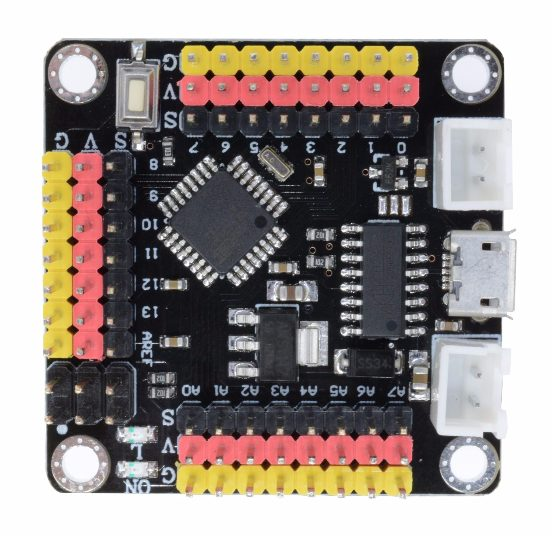
\includegraphics[width=0.4\textwidth]{images/arduino-nano-strong}}
\caption[Riadiaca jednotka - Arduino Nano Strong]{Riadiaca jednotka robota - Arduino Nano Strong}
\label{obr:arduino}
\end{figure}

\subsubsection{Programovanie mikropočítača Arduino}
Programovací jazyk Arduino je založený na jazyku C++, sú v ňom však navyše dostupné rôzne funkcie a knižnice umožňujúce ovládanie špecifických prvkov mikropočítača, najmä riadenie periférií, senzorov a motorov pomocou pinov \cite{ArduinoLanguage}. Periférie je teda možné jednoducho ovládať volaním príslušnej funkcie. K dispozícii je tiež voľne dostupný Arduino Software (IDE), v ktorom možno v textovom editore písať program, jedným kliknutím ho kompilovať, po pripojení USB kábla načítať do pamäte Arduina a spustiť. Program tvoria dve hlavné časti, metódy setup a loop. Metóda setup sa vykoná pri spustení programu práve raz, slúži predovšetkým na inicializáciu premenných, prípadne kalibráciu motorov, senzorov, určenie parametrov pinov a podobne. Metóda loop je následne vykonávaná v nekonečnom cykle, obsahuje hlavný program. S ohľadom na obmedzenia plynúce z veľkosti dostupnej pamäte je kód písaný v jazyku C++ zvyčajne čo najjednoduchší, s preferenciou jednoduchých štruktúr a pamäťovo úspornejších prvkov jazyka C.

\subsubsection{Komunikácia --- princíp}
S mikropočítačom možno komunikovať napríklad pripojením rozhrania USB. Výmena informácií je založená na asynchrónnej sériovej komunikácii. Bity v sériovej linke sú prenášané postupne, v každom smere v jednom kanáli, čo oproti paralelnej komunikácii, vyžadujúcej niekoľko vodičov, prináša výraznú úsporu zdrojov (dostupných pinov) mikropočítača. Asynchrónnosť tiež znižuje nároky na komunikačný kanál, nakoľko komunikujúce zariadenia nezdieľajú pripojenie zabezpečujúce zosúladenie hodín \cite{serialCommunication}. Úspory v tomto smere samozrejme nie sú bez následkov, prejavujú sa najmä v kvantite prenášaných dát, ku ktorým pribúda množstvo riadiacich informácií. Ich objem však nepredstavuje v tejto aplikácii prekážku, nakoľko ani samotné prenášané dáta nie sú zvyčajne rozsiahle.

Základom úspešnej asynchrónnej sériovej komunikácie je použitie rovnakého protokolu s rovnakými parametrami na oboch stranách. Ide najmä o prenosovú rýchlosť, počet bitov dát v pakete, počet synchronizačných (stop) bitov a určenie použitia bitu pre kontrolu parity. Pri komunikácii s mikropočítačom je štandardom rýchlosť 9600 bps, 8 bitov dát v pakete, jeden stop bit a informácia o parite (počtu kladných bitov v pakete) sa neprenáša \cite{serialCommunicationParameters}.

\subsubsection{Komunikácia zo strany mikropočítača}
Procesor mikropočítača rozpoznáva sériovú komunikáciu pomocou špecializovaného hardvéru --- UART \cite{sketchUpload}. UART (angl. Universal Asynchronous Receiver/Transmitter) prevádza paralelné dáta (zo zbernice CPU) do sériovej podoby \cite{uart}, pričom dve UART zariadenia sú schopné vzájomnej priamej sériovej komunikácie s použitím len dvoch prepojovacích vodičov. Činnosť UART je možné softvérovo simulovať a tak pripojiť i viacero takto komunikujúcich zariadení, aj na rôznych pinoch. Simuláciu môže uľahčiť knižnica \textit{SoftwareSerial} \cite{arduinoSoftwareSerial}.

V mikropočítači je sériový výstup UART vyvedený i na piny, takže možno ľahko priamo pripojiť i iné zariadenia (periférie) podporujúce tento štandard. Pre sériovú komunikáciu s počítačom prostredníctvom rozhrania USB je výstup z UART prepojený s \uv{USB-to-serial} čipom, ku ktorému existujú prislúchajúce ovládače pre OS. Činnosť tohto \uv{prevodníka} nemožno v mikropočítači softvérovo simulovať, v prípade potreby ich však možno pripojiť viacero (k simulovaným UART). V kóde je prístup k funkciám sériovej komunikácie umožnený objektom \textit{Serial} a jeho metódami (napríklad \textit{Serial.print()}, \textit{Serial.read()}, \textit{Serial.available()}). Komunikovať s perifériami možno i použitím protokolov ako SPI alebo I2C, ku ktorým sú tiež k dispozícii obslužné funkcie.

\subsubsection{Rozhranie Bluetooth}
Komunikovať s mikropočítačom možno aj prostredníctvom rozhrania Bluetooth, o ktoré bolo použité Arduino rozšírené \cite{PetrovicVaskoOtto}. Jeho zapojenie a implementácia ilustruje prípad softvérovej simulácie ďalšieho UART modulu. Pri konštrukcii robota vznikla táto nutnosť, nakoľko použitý mikropočítač disponuje jediným UART modulom, ktorý je využívaný pre komunikáciu s počítačom pripojením USB. Zapojenie modulu rozhrania Bluetooth (samostatná súčiastka) nemožno zlúčiť s existujúcim modulom UART, nakoľko potom dochádza k interferencii so sériovou komunikáciou prebiehajúcou cez USB (napríklad pri nahrávaní riadiaceho programu) \cite{PetrovicVaskoOtto}.


% Riadiaci program
\subsection{Riadiaci program}
Riadiaci program robota je vždy možné vytvoriť priamo ako program pre Arduino popísaný vyššie. V prípade denných táborov bolo ale zvolené iné riešenie, umožňujúce riadiť robota aj bez znalosti C++. Princíp je nasledovný. Riadiaci program napísaný v C++ prijíma počas behu, v časti loop, cez sériový port (pripojenie rozhraním USB alebo bezdrôtovou technológiou Bluetooth) postupnosť znakov, ktoré majú predurčený význam. Znaky rozpoznáva, a interpretuje ako príkazy. Na strane užívateľa je teda riadenie robota vykonávané zadávaním reťazca do znakového terminálu (napríklad prostredníctvom programu Putty v OS Windows). Popísaným spôsobom je možné riadiť robota manuálne ale i vytvárať jednoduché choreografie. Viac o programovaní a ovládaní uvádzame v častiach venovaných samostatným robotom, nakoľko ich možnosti nie sú totožné. Výhodou prístupu je mimo iného fakt, že pri ladení choreografie nie je potrebné zakaždým kompilovať program pre Arduino. Ústredným nedostatkom je na druhú stranu výraznejšie obmedzená dĺžka choreografie, keďže je nutné všetky jej prvky reprezentovať a uchovať v operačnej pamäti.

% Interakcia s prostredím
\subsection{Interakcia s prostredím}
Roboty interagujú s prostredím použitím receptorov, ktorými získavajú údaje z prostredia a efektorov, ktorými prostredie ovplyvňujú. K mikropočítaču Arduino možno pripojiť rôzne periférie. Aktuálna konštrukcia robotov Otto a Mokrarosa zdieľa použitie komponentov servomotor a ultrazvukový senzor.

Servomotor je typ motoru, ktorého úlohou väčšinou nie je kontinuálny pohyb (i keď nie je vylúčený) ale presné natočenie osi. Motor teda disponuje zariadením na určenie polohy, a na základe riadiacej informácie vždy prispôsobí svoje natočenie. V prípade robotov bolo pri stavbe použité mikroservo SG-90, umožňujúce nastavenie polohy v rozmedzí 180 stupňov. Pre riadenie je dostupná knižnica a nastavenie polohy jednotlivých motorov je tak v kóde len jednoduchým volaním príslušnej funkcie s parametrom definujúcim požadované natočenie.

Ultrazvukový senzor umožňuje bezkontaktne určiť vzdialenosť od prekážky, zisťuje ju podobne ako v prírode netopier. Princíp je založený na sonare, zariadenie pozostáva z vysielača vysokofrekvenčného (pre človeka nepočuteľného) zvuku a prijímača. Na začiatku merania je odvysielaný signál a následne sa čaká na jeho prijatie po odraze od prekážky. Dôležitý je práve časový rozstup vysielania a prijatia \uv{odrazeného} zvuku. Keďže rýchlosť šírenia zvuku vzduchom poznáme, vieme ľahko vypočítať prekonanú vzdialenosť za daný čas. Model použitý pri stavbe robotov nesie označenie HC-SR04.

% Otto
\subsection{Robot Otto}
\label{sub:otto}
Vznikol v rámci projektu Otto DIY v susednej Českej republike, s cieľom vytvoriť dostupného robota pre širokú verejnosť. Dnes je vyrábaných niekoľko verzii, robot je modulárny a všetok softvér a hardvér s ním spojený voľne dostupný v duchu open--source \cite{OttoDIY}. Otto bol ústrednou témou Denného tábora digitálnych technológií v roku 2018, kde sa ukázalo, že je vhodný pre demonštračné a edukačné účely pre začínajúcich programátorov. Modularita a open--source princíp sľubujú potenciál aj do budúcnosti, a aj preto je súčasťou našej práce.

\subsubsection{Konštrukcia, možnosti, schopnosti}
Vzhľadom sa snaží napodobniť človeka, má štyri končatiny, dve \uv{nohy}, každá poháňaná dvoma servomotormi, mu umožňujú pohyb do všetkých strán roviny. Môže tiež pohybovať \uv{rukami} v rozmedzí 180 stupňov, \uv{oči} tvorí ultrazvukový senzor schopný merať vzdialenosť od prekážky, zhora na hlave sú k dispozícii dve dotykové tlačidlá, ktoré možno použiť ako ďalšie vstupné zariadenie. V tele je osadený reproduktor a mp3 prehrávač. Robota Otto môžete vidieť na obrázku \ref{obr:otto}.

\begin{figure}
\centerline{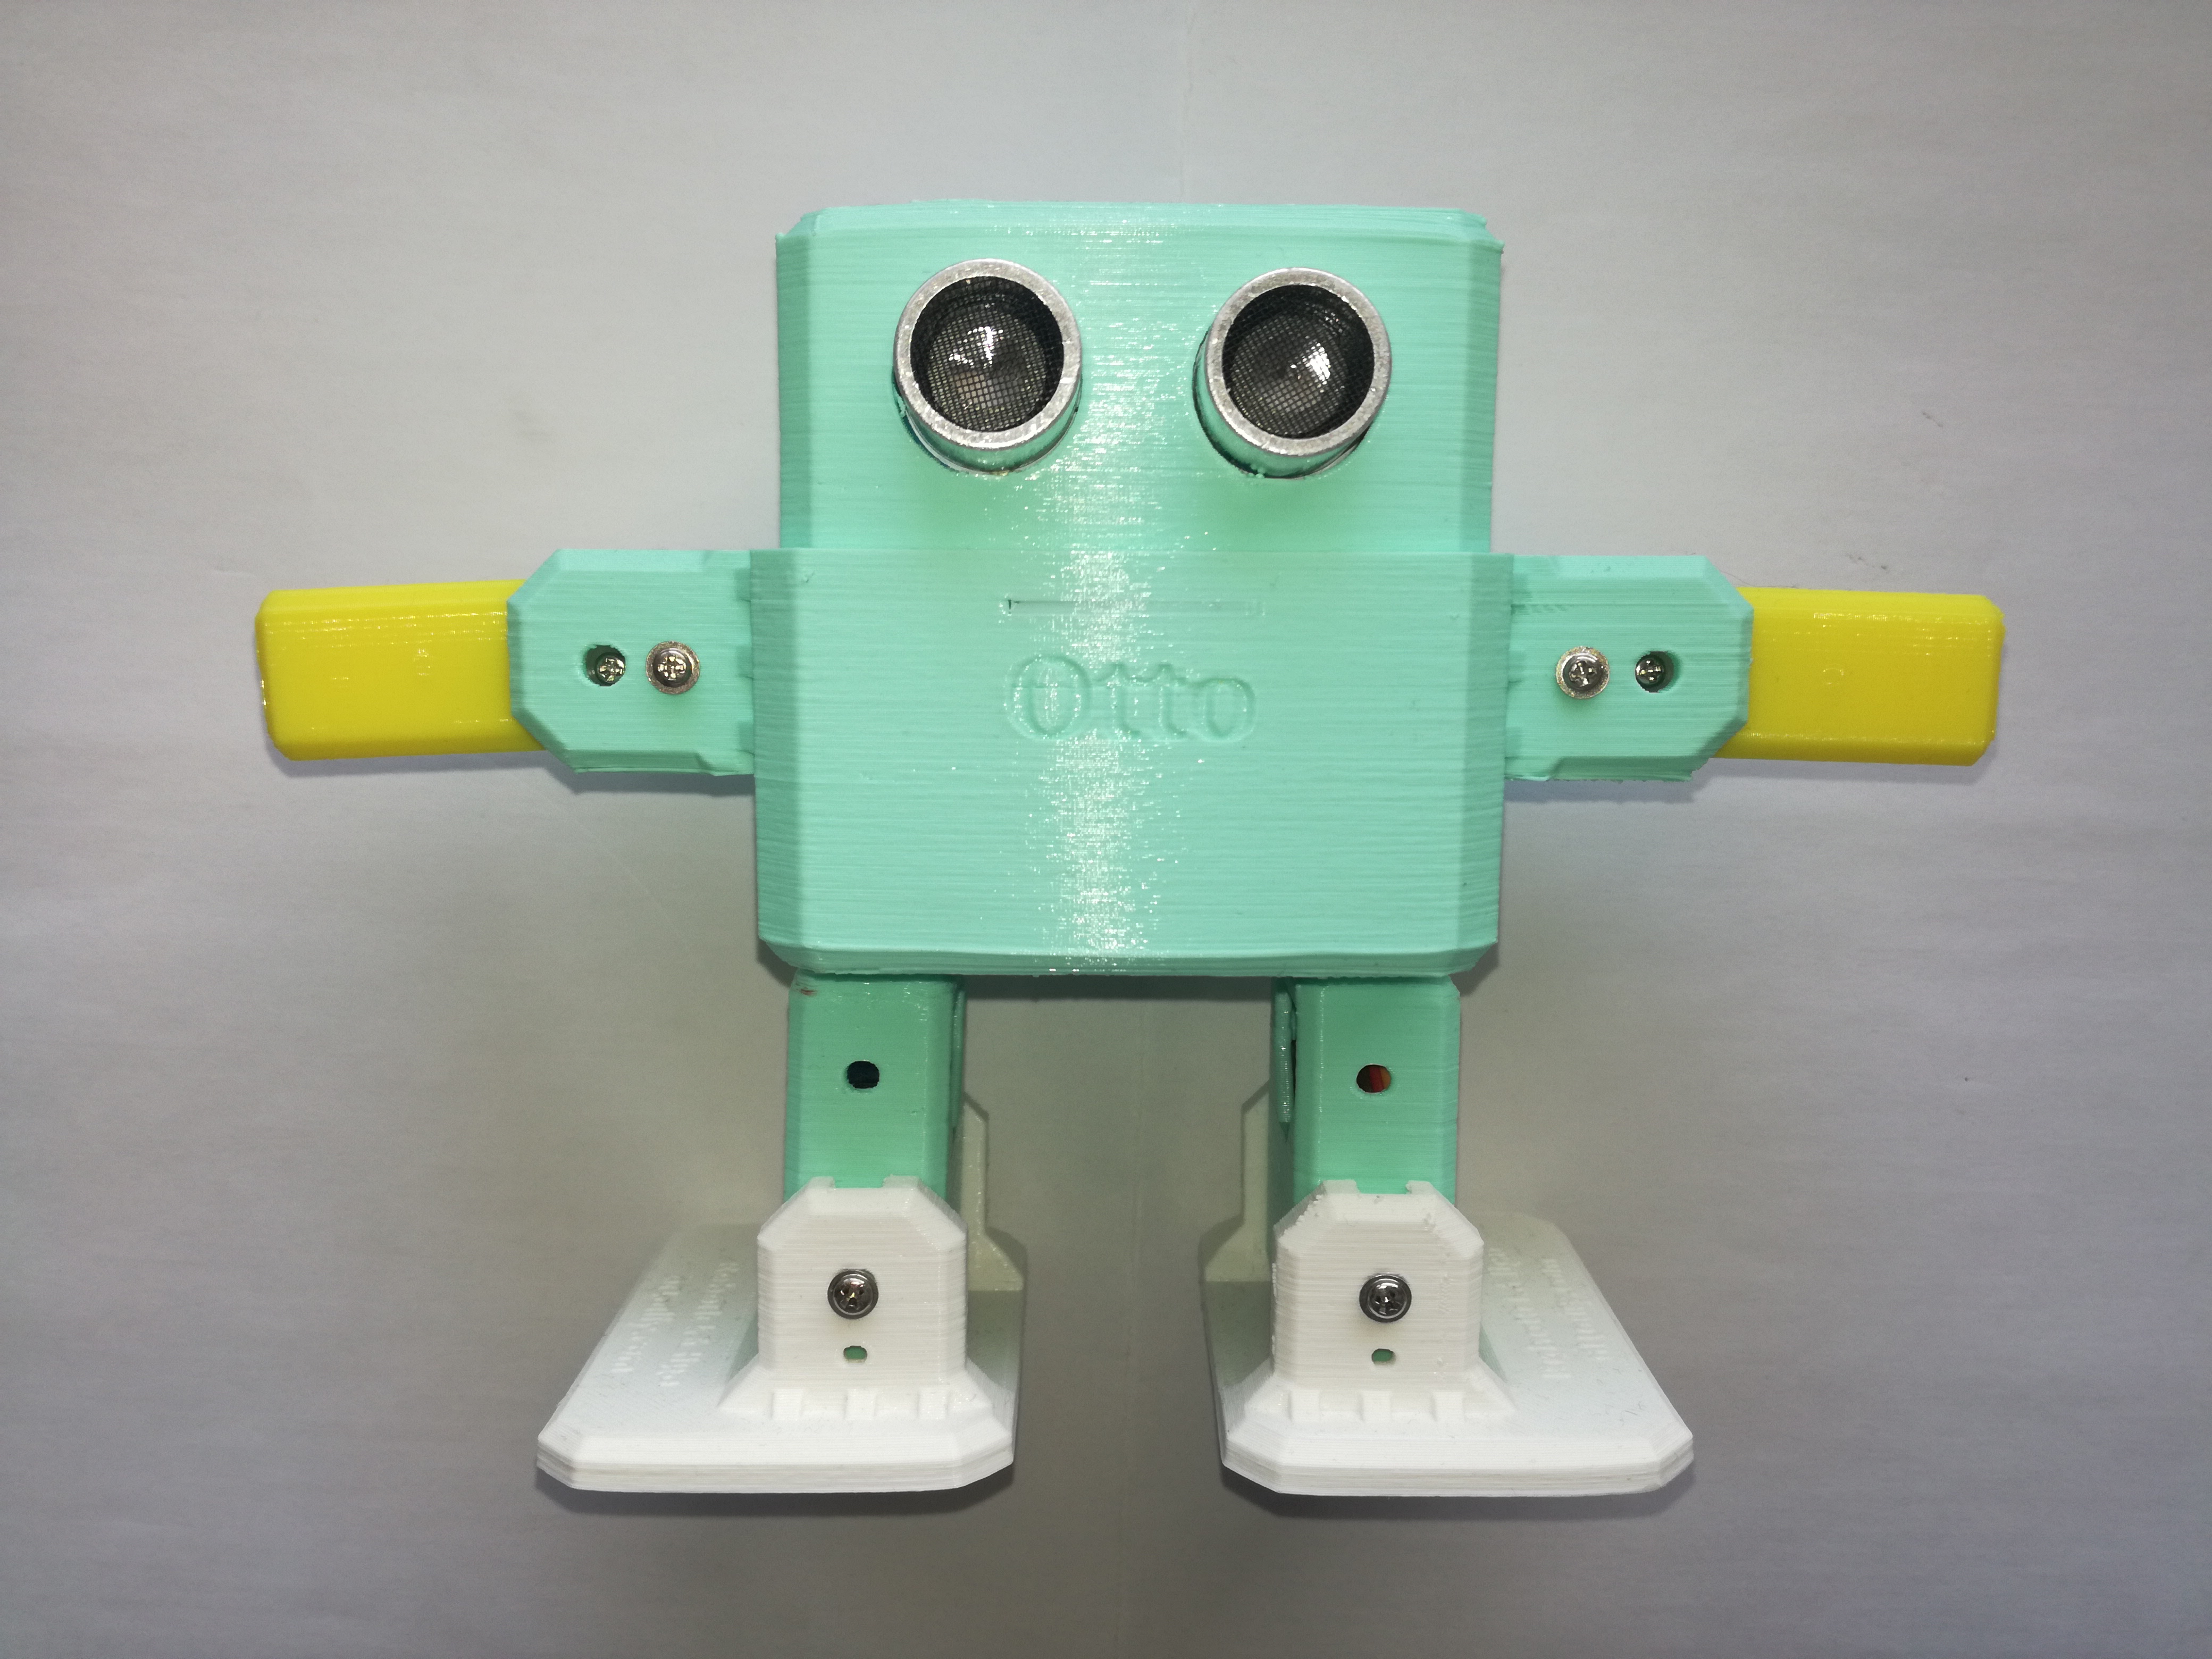
\includegraphics[width=0.4\textwidth]{images/otto}}
\caption[Robot Otto]{Robot Otto}
\label{obr:otto}
\end{figure}

\subsubsection{Riadiaci program, interakcia, programovanie}
\label{subsub:otto-programovanie}
Program vykonávaný Arduinom nie je prebraný od vynálezcov pôvodnej verzie robota. Vytvoril ho špeciálne pre účely denného tábora školiteľ tejto práce, Mgr. Pavel Petrovič, PhD. Ako spomíname v úvode, jedná sa o program umožňujúci programovanie robota bez znalosti C++. V najnovšej verzii (leto 2020) sú možné dva varianty interakcie s robotom.

Robota možno ovládať priamo. V tomto režime zariadenie vykonáva príkazy (znaky) prijaté cez sériový port ihneď. (Príkazy sú v komunikácii reprezentované znakmi a riadiaci program ich po prečítaní interpretuje ako príkazy.) Takéto povely sú charakteru \uv{posuň motor A do polohy X} alebo \uv{pípni}. Možno tiež spustiť prehrávanie niektorej z predprogramovaných melódií alebo choreografií, ovládať mp3 prehrávač, kalibrovať pozície servomotorov a vytvorenú kalibráciu uložiť do pamäte EEPROM.

Druhým prístupom je programovanie choreografií a ich následné spúšťanie. Jedným z interpretovaných znakov --- príkazov je aj špeciálny znak na prechod do režimu programovania. Tu je možné zadať program ako postupnosť trojíc (doba čakania v milisekundách, číslo motora, rotácia motora v stupňoch) a niekoľkých špeciálnych príkazov (tiež ako trojice), ktoré umožňujú napríklad \uv{skoky} v programe (v podstate inštrukcia jump --- vykonávanie programu pokračuje zadaným riadkom kódu, za čo sa považuje každá takáto trojica). Súčasťou sú tiež trojice --- inštrukcie na prehranie melódie, prípadne zvukového efektu. Takto vytvorený program je ukladaný do pamäte RAM, v riadiacom programe vykonávanom v mikropočítači sú spomínané trojice reprezentované ako prvky poľa celých čísel. Programovanie je teda značne limitované veľkosťou pamäte a často neprehľadné. Upraviť nahraný program nie je možné priamo v mikropočítači, je nutné nahrať nový, čo v prípade ladenia choreografie môže znamenať časté, nepraktické prepínanie medzi terminálom a textovým editorom. Výhodou však stále bezpochyby zostáva možnosť interakcie s robotom a tvorby choreografie bez znalosti C++ a tiež bez nutnosti kompilácie a nahratia riadiaceho programu pri zmene kompozície pohybov.

\newpage

% Mokrarosa
\subsection{Robot Mokrarosa}
Robot MoKraRosA (MOdulárny KRAhulský RObot S Arduinom) bol témou Denného tábora digitálnych technológií v roku 2019 \cite{PetrovicVaskoMokrarosa}. Vyvinutý je od základu v dielni Fablab Bratislava kde bolo toho roku skonštruovaných 80 kusov s podobným cieľom ako predtým robot Otto \cite{Mokrarosa}.

\subsubsection{Konštrukcia, možnosti, schopnosti}
Telo robota Mokrarosa pripomína pavúka (obrázok \ref{obr:mokrarosa}). Aj tu bol použitý rovnaký modul pre senzor merania vzdialenosti od prekážky ktorý v dizajne imituje \uv{oči} prístroja. Pavúk je navyše osadený gyroskopom, ktorý mu umožňuje reagovať na preklopenie, prípadne pád. Konštrukcia dovoľuje nohami robota prevrátiť alebo vykonať kotúľ, pričom na základe údajov z gyroskopu môže vždy nasmerovať' nohy smerom k zemi a tak sa nikdy nedostane do polohy, z ktorej by nebol možný pohyb (na rozdiel od robota Otto). Štandardne je tiež osadený mp3 prehrávačom a reproduktorom.

\begin{figure}
\centerline{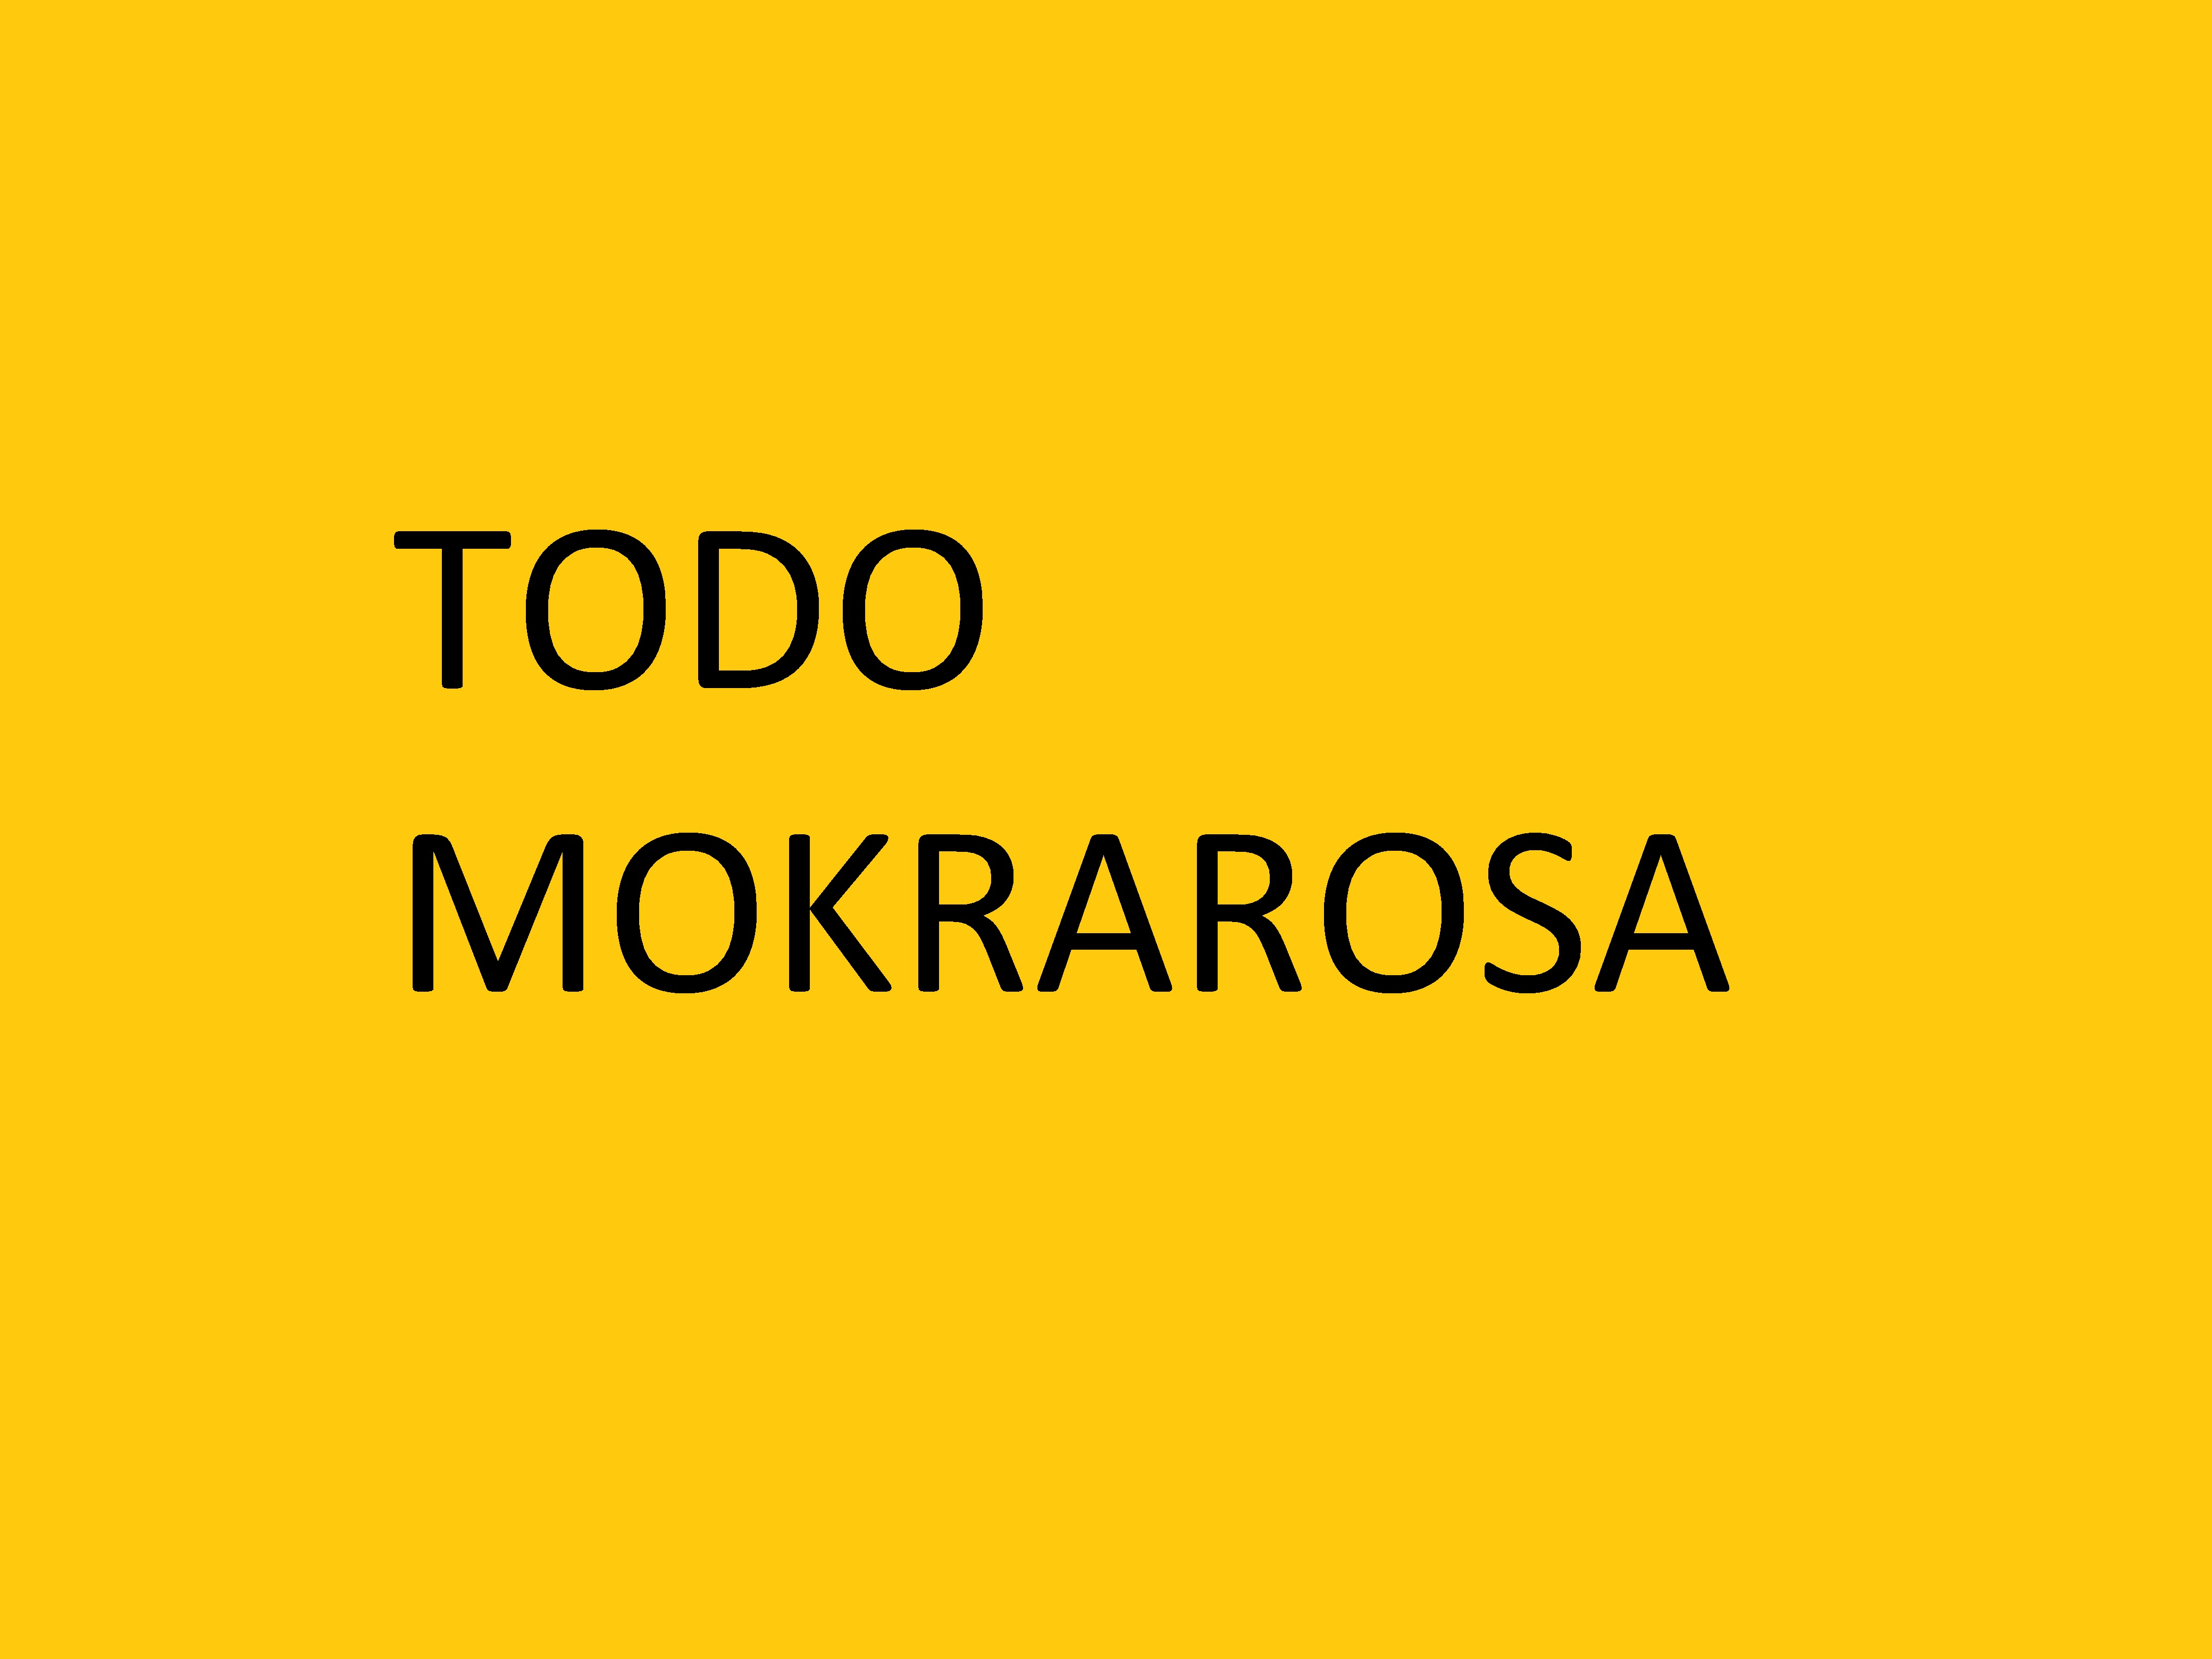
\includegraphics[width=0.4\textwidth]{images/mokrarosa}}
\caption[Robot Mokrarosa]{Robot Mokrarosa}
\label{obr:mokrarosa}
\end{figure}

\subsubsection{Riadiaci program, interakcia, programovanie}
Riadiaci program pavúka je o niečo zložitejší. Umožňuje jednak robota riadiť \uv{po znakoch}, v tomto móde ihneď reaguje na symbol prijatý cez sériový port, obdobne ako v prípade robota Otto. V režime programovania sa výraznejšie líši. Program je daný ako postupnosť n-tíc kde každá n-tica vyjadruje v akej polohe (v stupňoch) sa má v daný moment daný motor nachádzať. Je tak možné hýbať s viacerými motormi naraz. Podstatný rozdiel je tiež v postupe programovania. Program je možné tvoriť tak, že robota postupne navádzame v režime \uv{po znakoch}, teda manuálnym pohybom jednotlivými motormi, do požadovanej polohy a následne uložíme stav --- natočenie každého z motorov do spomínanej n-tice. Takto postupne vytvárame \uv{pózy} --- konfigurácie, cez ktoré robot následne plynule prechádza. Vytvorenú choreografiu možno opakovane ladiť krokovaním a úpravou vybranej konfigurácie.

% ===
% === Existujúce riešenia
% ===
\section{Existujúce riešenia}
Jediné nám známe dostupné príbuzné riešenie súvisí s robotom Otto. Pochádza priamo od jeho tvorcov, ktorí vyvinuli pomerne rozsiahlu aplikáciu na tvorbu riadiacich programov. V prípade robota Mokrarosa podobné riešenia pochopiteľne neexistujú, nakoľko je len nedávnym produktom dielne Fablab Bratislava. Uvádzame však i iné produkty súvisiace s výučbou robotiky a programovaním robotov.

\subsection{Otto Blockly}
\label{sub:OttoBlockly}
Ide o desktopovú aplikáciu z produkcie konštruktérov robota Otto, umožňujúcu programovať robota v grafickom jazyku, vytvorenom pomocou knižnice Google Blockly \cite{OttoBlockly}. Produktom sa možno vo viacerých aspektoch inšpirovať. Aplikácia je profesionálne graficky spracovaná, podporuje rôzne funkcie robota, ponúka okamžitý preklad vytvoreného kódu riadiaceho programu do C++, ktorý možno ľahko kompilovať a nahrať priamo do pripojeného mikropočítača Arduino. V grafickom jazyku sú k dispozícii prvky ovládajúce pokročilé funkcie rôznych verzií robota. Súčasťou sú predpripravené ukážkové kódy a tiež možnosť komunikácie cez sériový port. V čase vzniku tohto textu je k dispozícii verzia 1.3.0.

Nevýhodou pre nás je predovšetkým naviazanosť na robota z výroby autorov. Nami používaný klon robota Otto je modifikovaný, a tak by pre použitie s aplikáciou bolo potrebné s každou zmenou zapojenia zmeniť aj logiku generátora kódu v aplikácii. Rovnako aplikácia nepodporuje štýl programovania kde sú vytvárané choreografie ukladané bez potreby kompilácie do pamäte RAM. Tento prístup je pritom mimoriadne výhodný pri častom ladení jednoduchých choreografii. Našim cieľom je vytvoriť alternatívny, nezávislý softvér, ktorého životný cyklus, dynamika a rozšíriteľnosť nie je naviazaná na spomínaný projekt.

\subsection{Lego Mindstorms}
\label{sub:LegoMindstorms}
Jedná sa o komplexnú stavebnicu umožňujúcu stavbu a programovanie robota \cite{LegoMindstormsEducationSet}. Základom je riadiaca jednotka, do ktorej možno pripájať senzory a motory, avšak ich počet je v základnej verzii limitovaný dostupnými portami na maximálne štyri motory a štyri senzory, možno však dokúpiť (neoficiálne) \uv{rozbočky} a zapojiť i väčší počet. K stavebnici možno pripojiť rôzne receptory, gyroskop, kompas, svetelný či ultrazvukový senzor. Všetky periférie sú s riadiacou jednotkou spojené vodičmi zakončeniami pripomínajúcimi telefónne káble. Modularita systému je ohraničená dostupnými produktmi ponúkanými firmou Lego, výber je rozmanitý, no komponenty nie sú až tak cenovo prívetivé. Pre porovnanie uvádzame cenu ultrazvukového senzora --- Lego senzor 34,99€ \cite{LegoMindstormsUltrasonic} a senzor použitý pri stavbe robota Otto 0,70€ \cite{OttoUltrasonic}.

K hardvéru ponúka Lego i prislúchajúci softvér na tvorbu riadiacich programov. Oficiálna aplikácia umožňuje programovanie vo vizuálnom jazyku, kde používateľ v grafickom rozhraní vytvára kód ako postupnosť ikon, prvkov reprezentujúcich senzory, motory ale napríklad i cykly. Ikony možno konfigurovať a tak nastavovať parametre ikonou reprezentovaného úkonu. Ikona \uv{pohyb motora} má napríklad parametre ako port, v ktorom je zapojený motor, rýchlosť, smer a miera otočenia.

Plynulý prechod programátorov od grafických jazykov k bežným textovým v prípade robotov rady Mindstorms umožňujú rôzne alternatívne programovacie platformy, kde možno riadiaci program tvoriť v jazyku Python (EV3Python) či C (RobotC) \cite{LegoAlternatives}.










